\documentclass[11pt,a4paper,final]{article}

\usepackage{notes}
\usepackage{float}
    
\title{Geophysics IIIA}
\author{Practical: Gravity Methods}

\begin{document}
\maketitle

The objectives of this practical are to
\begin{itemize}
    \item introduce you to a relative gravimeter
    \item gravity anomalies
    \item estimate density from observations of rock mineralogy
    \item measure density
\end{itemize}
You will be working in small groups to do these exercises.

\section*{Problem 1 --- Density Estimates versus Measurements\hfill [10 pts.]}
Obtain igneous rocks of differing compositions.  You will be measuring and estimating the theoretical density of these rocks following the procedures below.

\subsection*{A) Mineralogy-based estimates}
Make a table of rock samples and the minerals listed in the table of mineral densities below.
\begin{enumerate}
    \item Start by estimating the density of your rock. Use the chart of grain percentages provided to estimate the mineralogical composition of your samples.  Start by estimating the percentage of dark minerals as they are easiest to spot.  Estimate from low percentage minerals to high percentage minerals.  Note the sum must be 100\% so adjust your estimates accordingly.  If your rock is igneous, use the chart below to identify whether it is felsic, intermediate, mafic or ultramafic.
        \begin{figure}[hbt]
          \centering
          
\includegraphics[angle=90]{figures/igneous_rock_minerals.eps}
          \caption{Mineralogical compositions of igneous rocks.}
          \label{fig:igrock}
        \end{figure}

    \item Compute the density of your rock by using the percentages you just determined and the table of mineral densities below.  If you don't see the minerals you need, there is a larger list at the end of your gravity lecture notes.
    \begin{table}[hbt]
        \footnotesize
        \centering{
        \caption{Mineral densities in kg~m$^{-3}$.\vspace{2pt}}
        \label{tab-mindensity}
        \begin{tabular}{lc}
            \toprule
            \textbf{Mineral} &
            \textbf{Density} (\si{kg.m^{-3}}) \\
            \midrule
            quartz           & 2648 \\
            orthoclase       & 2555 \\
            plagioclase      & 2731 \\
            muscovite        & 2635 \\
            biotite          & 3317 \\
            amphibole        & 3248 \\
            pyroxene         & 3360 \\
            olivine          & 3472 \\
            serpentine       & 2300 \\
            garnet           & 4320 \\
            omphacite        & 3300 \\
            pyrite           & 5020 \\
            galena           & 7500 \\
            magnetite        & 5180 \\
            \bottomrule
        \end{tabular}
        }
    \end{table}
\end{enumerate}

\subsection*{B) Hydrostatic weighing}
\begin{enumerate}
    \item This method employs Archimedes' principle to estimate the density by fluid displacement.
    \begin{enumerate}
        \item Record the dry mass of the rock sample, $m_{\mathrm{dry}}$.

        \item Record the wet mass of your rock sample, $m_{\mathrm{wet}}$ by supporting the rock in the strings attached to the balance.  Before recording this mass, ensure that your sample does not touch the bottom or sides of the reservoir and is completely submerged.
        
        \item Compute the specific gravity by
        \begin{equation}
            \frac{\rho_{\mathrm{rock}}}{\rho_{\mathrm{water}}} =
            \frac{m_{\mathrm{dry}}}{m_{\mathrm{dry}} - m_{\mathrm{wet}}} ,
        \end{equation}
        where $\rho$ is density and $m$ is mass.  Note: since specific gravity
        is the rock density relative to water the result is unitless.

        \item Multiply by the density of water to obtain the rock density, $\rho_{\mathrm{rock}}$. At 21 $^\circ$C, the approximate temperature in the room, water has a density of 998 kg m$^{-3}$.
    \end{enumerate}

    \item We could have estimated density by measuring the mass and then measuring the volume displaced by submurging the sample in water.  However, this is far less accurate than the hydrostatic technique. Why do you think this may be the case?

    \item How do your measured densities compare with your mineral-based estimates?  If they are different by more than a few percent, why do you think this happened?  Is it related to your compositional estimates or the specific to the rock sample?  How could you test your answer?

    \item How does the relative felsic versus mafic nature of the rock affect the density?  What does this tell you about the density as you move deeper into Earth?
\end{enumerate}

\begin{table}[hbt]
\begin{tabularx}{\textwidth}{|X|Y|Y|Y|Y|Y|}
    \multicolumn{6}{c}{Density measurements} \\
    \toprule
    \textbf{Sample} &
    $m_{\mathrm{dry}}$ (g) &
    $m_{\mathrm{wet}}$ (g) &
    $\rho_{\mathrm{rock}}/\rho_{\mathrm{water}}$&
    $\rho_{\mathrm{water}}$ (kg~m$^{-3}$) &
    $\rho_{\mathrm{rock}}$ (kg~m$^{-3}$) \\
    \midrule
    1. & {} & {} & {} & 998 & {} \\
    \midrule
    2. & {} & {} & {} & 998 & {} \\
    \midrule
    3. & {} & {} & {} & 998 & {} \\
    \midrule
    4. & {} & {} & {} & 998 & {} \\
    \midrule
    5. & {} & {} & {} & 998 & {} \\
    \bottomrule
\end{tabularx}
\end{table}

\clearpage

\section*{Problem 2 --- Free-air correction\hfill [10 pts.]}
{\bf Read all instructions before making a single measurement.} For this problem, we will investigate the free-air gravity correction by making measurements on several levels of a building above the same point.  By making observations at the same point only at different levels, we can ignore all the other corrections that we would normally make.

{\bf Note:} Gravimeters are fragile instruments and can easily break if mistreated.  {\it The gravimeters must remain in the sensor clamped position unless a reading is in progress.}

The gravimeters that we will use were made by Lacoste and Romberg and were for many years the industry standard.  A trained user can take nearly as accurate a reading with these meters as the newer electronic meters.
\begin{figure}[hbt]
    \centering
    \includegraphics[width=6.14in]{figures/gravimeter.eps}
    \caption{A Lacoste and Romberg gravimeter.}
    \label{fig:gmeter}
\end{figure}
\FloatBarrier
\begin{enumerate}
    \item Before moving the gravimeter, ensure that the meter is clamped (turn clockwise as until you hit the stop).

    \item Grabbing the meter by the thumb screws, gently remove the gravimeter from the case.  Place your hand under and on the sides of the meter as soon as possible for the most stable handling.

    \item Place the gravimeter on the base plate (if you have one) above the measurement mark.  The base plate isn't actually needed in a building, but the measurement procedure should be followed exactly the same each time to ensure the most accurate measurements.

    \item Using the thumb screws, level the meter.  Work on leveling the axis defined by the pair of thumbscrews on the left.  Once this axis is level, use remaining screw to level the second axis.  This process may be iterative.

    \item Next, flip the switch on the gravimeter to turn the lights on and unclamp the meter.  Look down the scope.  If the measurement bar is to the left of the reading line, increase counter by turning it counter-clockwise.  Turn the dial until the measurement bar is above the reading line.

    We will always approach the reading line from the same side to remove the error due to backlash in the screws.  In this case the high (or right) side of the reading line.

    Once the measurement bar is to the right of the reading line reduce the counter by turning the dial clockwise.

    If the dial reading is far from the correct gravity measurement, then turning the dial will seem like it isn't doing anything.  Once you get get close to the range of the scale you might see the measurement bar bounce a couple times.  At this point turn the dial more slowly.  As you approach the reading line, use small turns and occasionally wait for the measurement bar to catch up.  Because it is controlled by a spring (albeit damped), there is a delay in the movement of the measurement bar.
    
    While peering down the scope, slowly adjust the dial until the left side of the measurement bar just kisses the right hand side of the measurement bar.  See figure~\ref{fig:rl}.
    \begin{figure}[hbt]
        \centering
        \includegraphics[]{figures/reading_line.eps}
        \caption{Reading line.  Approach the reading line from the right until
        the measurement bar just touches the reading line.  In this case 2.2.}
        \label{fig:rl}
    \end{figure}
    \FloatBarrier

    \item At this point, record the value of the counter.  The last digit should duplicate the dial.  Read this number off of the dial, the tick mark just below the pointer and estimate the position of the measuring point between the two tick marks.  This is the last value that is recorded and the uncertain digit. See the example in Fig.~\ref{fig:dial}.
    \begin{figure}[hbt]
        \centering
        \includegraphics[]{figures/dial.eps}
        \caption{How to read a gravimeter dial. Read the counter next to the wheel first.  The last digit of the wheel is uncertain.  When reading the wheel read the number before reading point, then read the last tick before the line and estimate the location of the point between ticks.  In this case the gravity reading is 3057.068.  Note the 8 is uncertain and must be estimated but if you are good, you can be consistently precise in measurement of this last digit.}
        \label{fig:dial}
    \end{figure}

    \item Clamp the meter.  You may now repeat the measuring procedure above on each floor.
\end{enumerate}

\clearpage
\subsection*{A) Free-air derivation}
Derive the free air gravity correction at the surface of the Earth (mean radius \(R_{\oplus} = 6371\)~km).  You may do so with or without a derivative. This derivation can be done with or without calculus.  The starting point is the gravitational acceleration of a sphere,
\[
    g = \frac{GM_{\oplus}}{r^2}
\]

\subsection*{B) Free-air observations}
Use observations collected this year along with past observations to estimate the free air correction.

You will start with an Excel spreadsheet (see course website) that looks like the table below.  Your task is to complete the table and compute the mean and standard deviation for the measurements and make a histogram of the values.
\begin{table}
    \caption{Free-air gravity worksheet.}
    \label{tab:fa}
    \begin{tabularx}{\textwidth}{|X|Y|Y|Y|Y|Y|Y|}
        \toprule
        \textbf{Floor} &
        $\Delta h$ &
        \textbf{dial counts} &
        \textbf{calibration \newline factor} &
        $g_{z}$ (\si{mgal}) &
        $\Delta g_{z} = g_{z} - g_{z,1}$ (\si{mgal}) &
        $g_{fa} = \Delta g_{z} / \Delta h$ (\si{mgal.m^{-1}})\\
        \bottomrule
    \end{tabularx}
\end{table}
For each year that measurements were made,
\begin{enumerate}
    \item Compute the height difference between the floors of successive measurements, e.g. if the first measurement was on floor 1 and the second on floor 3, compute the distance between floors 1 and 3.
    
    \item Convert from dial counts to a relative mGal value using the meter calibration factors.

    \item Compute the difference in gravity between successive floors, $\Delta g_{z}$. Note: you cannot estimate the gravity difference across years unless corrections were made for instrument drift and Earth tides, neither of which have been done.

    \item Divide the change in gravity by difference in heights to obtain an estimate of the free-air correction, $\Delta g_{fa}$.
    
    \item Compute the average and standard deviation of your measurements.  Make sure to exclude clear outliers from the calculation.
\end{enumerate}

For both the measured values and the theoretical calculation you should get a decrease in gravity of approximately 0.3086 mGal m$^{-1}$.  How do your results, $\Delta g_{fa}$, compare with the free-air gravity correction and the theoretical calculation?  What might be some reasons for the differences?

\section*{Problem 3 --- Back of the Envelope\hfill [10 pts.]}
What change in water table height results in a gravity anomaly of 10~\(\mu\)Gal?

Hints:
\begin{itemize}
    \item You will need the equation for a Bouguer slab (\(g_{\text{\it bs}} = 2 \pi G \Delta \rho h\)).
    \item The density contrast is not simply the density of the water.
\end{itemize}

Does it matter what depth below the surface the water table sits? If so, how? And if not, why not?

\section*{Problem 4 --- Buried Sphere\hfill [10 pts.]} \label{itm:sphere} 
In this problem, we'll be exploring the buried sphere that we have used in several contexts so far.
\begin{figure}[H]
    \centering
    
\includegraphics{figures/buried_sphere.eps}
    \caption{Buried sphere setup.}
    \label{fig:bs}
\end{figure}
\begin{enumerate}
    \item Reformulate the gravitational potential for a buried sphere,
    \[
        U(R) = -\frac{4}{3} \pi G \Delta \rho \frac{a^3}{R},
    \]
    in Cartesian coordinates with the depth to the center of the sphere, \(z\),
    and at a distance from the center \(x\) along the surface from the center of
    the sphere.  Assume the sphere has a radius, \(a\), and a density contrast
    with the surrounding rock, \(\Delta \rho\).

    \item Take the vertical derivative of the potential, \(\pd{U}{z}\) to find the gravity anomaly
    \(g_{z}\).

    \item Graph the previous result.  Make sure you label the axes.

    \item If the sphere now has a radius of \(2a\), what must the density contrast be for the gravity anomaly to be the same?

    \item Develop a formula that relates the depth to the full-width at half-maximum (FWHM) of the anomaly.  Hint: take your formula for the gravity due to a buried sphere and find \(g_z(x_{1/2}) = \frac{1}{2} g_z(0)\), where \(x_{1/2}\) is the location where the gravity is half the peak value.  Solve for depth relative to \(x_{1/2}\) and divide by two to determine your the relationship to the FWHM.

    \end{enumerate}

\end{document}